\documentclass[ngerman]{gdb-aufgabenblatt}

\usepackage{enumitem}
\usepackage{dingbat}
\usepackage{ifsym}
\usepackage{amssymb}
\usepackage{amsmath}
\renewcommand{\Aufgabenblatt}{3}
\renewcommand{\Ausgabedatum}{Mi. 15.11.2017}
\renewcommand{\Abgabedatum}{Fr. 01.12.2017}
\renewcommand{\Gruppe}{Meimerstorf,Jochens,T�ter}
\renewcommand{\STiNEGruppe}{19}
\usepackage{tabularx}


\begin{document}

\begin{center}
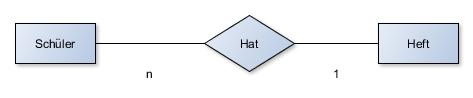
\includegraphics[scale=0.3]{RelationShipBeispiel.jpg} \ \\
\end{center}

Am Anfang kurz definiert wie die Relationen zu lesen sind. So wie es in der Vorlesung vorgestellt wurde. \\
1 Kind kann n Hefte haben. \\
Ein Heft kann nur von einem Kind bessen werden \\
\section{Informationsmodellierung mit dem Entity-Relationship Modell}
\subsection{}
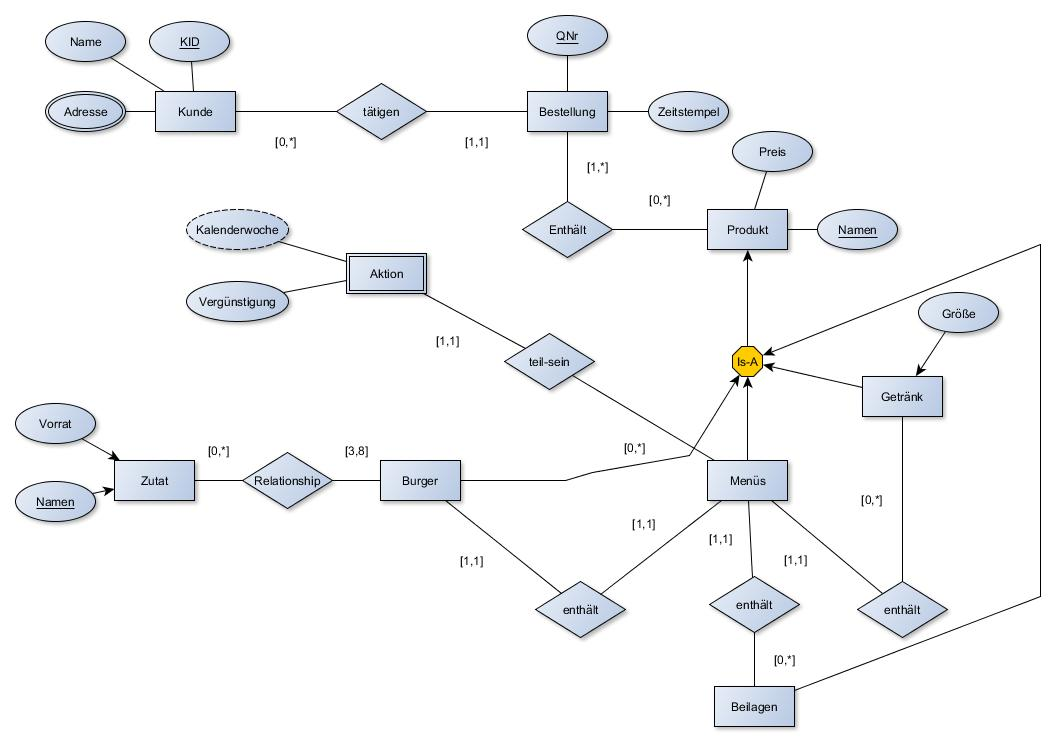
\includegraphics[scale=0.5]{GraphAufgabe3.jpg}
Anmerkung: Kalenderwoche soll eigentlich gestrichelt unterstrichen sein, da es nur mit dem Namen eindeutig ist, dies war in Yed Graph Editor jedoch nicht m�glich
\section{}
\section{Relationale Algebra}
\subsection{}
\subsubsection{}
Die erste Aussage ist nicht korrekt, da in der letzten Selektion 
$\sigma_{Geburt=1962-07-25}$ ein Attribut abgefragt wird, welches in der ersten Projektion $\pi_{PID,Vorname,Nachname}$ bereits rausgefiltert wurde. \\
\subsubsection{}
Ist korrekt.
\subsubsection{}
Syntaktisch korrekt, macht jedoch semantisch kein Sinn durch die Bedingung $Budget < 1000 \wedge Budget > 5000$ da diese Bedingung niemals erf�llt werden kann. \\
\subsubsection{}
Nicht korrekt, da in dem Join Attribute abgefragt werden, die allerdings schon von den Projektionen rausgenommen werden. \\
\subsection{}
\subsubsection{}
$ \pi_{Name}(Projekte \bowtie ProjektArbeiter \bowtie \sigma_{Geburt>01.01.1990}(Personal))$\\
$L=\lbrace("B.L.I.C.K.F.A.N.G.")\rbrace$ \\
\subsubsection{}
$\pi_{Vorname,Nachname,Geburt}(\sigma_{Name=Prozessoptimierung}(Projekte) \bowtie ProjektArbeiter \bowtie Personal))$ \\
$L=\lbrace(Frank,Siebenstein,1975-12-02),(Bernd,Schmidt,1973-11-26)\rbrace$ 
\subsubsection{}
$Personal  \setminus  \pi_{PID,Vorname,Nachname,Geburt,Wohnort,Abteilung}(ProjektArb \verbund{ProjektArb.PID=Personal.PID} Personal)$ \\
$L=\lbrace(4,Peter,Mueller,1962-07-25,Hamburg,2),(24,Ulrike,Mueller,1963-10-07,Hamburg,2
)\rbrace$ 
\subsubsection{}
\begin{small}
$\small \pi_{Vorname,Nachname}\sigma_{Nachname \neq Fuhrmann \wedge Vorname \neq Jochen}(Personal \underset{A.Abteilung=B.Abteilung}{\ltimes} \sigma_{Nachname = Fuhrmann  \wedge Vorname = Jochen} (Personal))$
\end{small}
$L=\lbrace (Ulrike,Mueller),(Murat,Sahir),(Peter,Mueller) \rbrace$
\subsection{}
\subsubsection{}
Die Vornamen und Nachnamen aller Leiter von Projekten deren Budget mehr als 8000 ist. \\
$L=\lbrace (Bernd,Schmidt) \rbrace$
\subsubsection{}
Alle Projektleiter und Abteilungsleiter \\
$L=\lbrace (4, Peter ,Mueller, 1962-07-25, Hamburg, 2
),(8 ,Bianca Lohse ,1982-01-13 ,Kiel ,4
), (21 ,Frank, Siebenstein ,1975-12-02, Norderstedt, 1),(22, Bernd ,Schmidt, 1973-11-26, Norderstedt ,1)  \rbrace$ 
\subsubsection{}
Die Namen der Abteilungen, in denen sich die Mitarbeiter von Projekt B.L.I.C.K.F.A.N.G., befinden. \\
$L=\lbrace (Marketing),(Einkauf) \rbrace$
\subsubsection{}
Die Projekte in denen die Mitarbeiter der Abteilung Controlling mitarbeiten.\\
$L= \lbrace (15,Prozessoptimierung,22,10.000)$
\section{}
\subsection{}
\begin{center}
\begin{tikzpicture}[scale=0.2]
\tikzstyle{every node}+=[inner sep=0pt]
\draw (33.8,-16.1) node {$\sigma_{Leiter=22}$};
\draw (33.7,-22.9) node {$\verbund{}$};
\draw (25.5,-30.2) node {$\verbund{}$};
\draw (17.2,-38.4) node {$Personal$};
\draw (33.7,-9.1) node {$\sigma_{Nachname=Meier}$};
\draw (30.5,-38.4) node {$ProjektArb$};
\draw (42.8,-37.4) node {$Projekt$};
\draw (33.7,-2.1) node {$\pi_{PID,Vorname,Nachname}$};
\draw [black] (31.46,-24.89) -- (27.74,-28.21);
\draw [black] (33.76,-19.1) -- (33.74,-19.9);
\draw [black] (33.74,-12.1) -- (33.76,-13.1);
\draw [black] (28.94,-35.84) -- (27.06,-32.76);
\draw [black] (19.33,-36.29) -- (23.37,-32.31);
\draw [black] (41.21,-34.86) -- (35.29,-25.44);
\draw [black] (33.7,-5.1) -- (33.7,-6.1);
\end{tikzpicture}
\end{center}
\subsection{}


\begin{center}
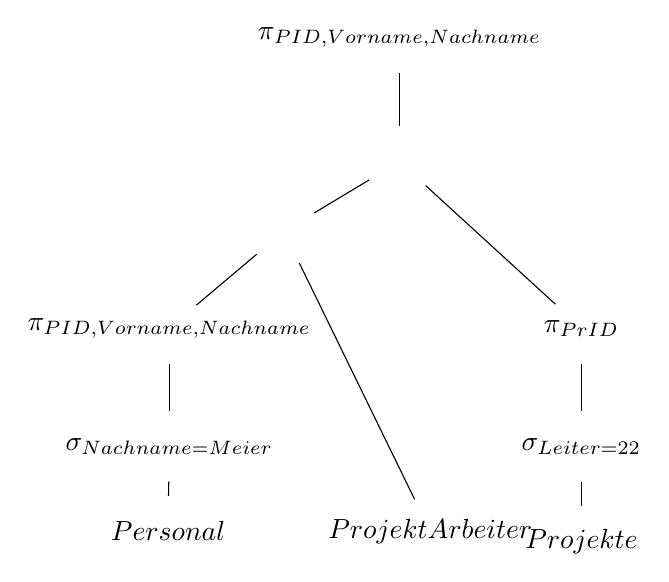
\begin{tikzpicture}[scale=0.15]
\tikzstyle{every node}+=[inner sep=0pt]
\draw (13.4,-50.9) node {$Personal$};
\draw (35.6,-50.9) node {$ProjektArbeiter$};
\draw (48.4,-51.8) node {$Projekte$};
\draw (48.4,-43.7) node {$\sigma_{Leiter=22}$};
\draw (48.4,-33.7) node {$\pi_{PrID}$};
\draw (13.5,-43.7) node {$\sigma_{Nachname=Meier}$};
\draw (13.5,-33.7) node {$\pi_{PID,Vorname,Nachname}$};
\draw (23.2,-25.5) node {$\verbund{}$};
\draw (33,-9.1) node {$\pi_{PID,Vorname,Nachname}$};
\draw (33,-19.6) node {$\verbund{}$};
\draw [black] (48.4,-46.7) -- (48.4,-48.8);
\draw [black] (48.4,-36.7) -- (48.4,-40.7);
\draw [black] (13.46,-46.7) -- (13.44,-47.9);
\draw [black] (13.5,-36.7) -- (13.5,-40.7);
\draw [black] (20.91,-27.44) -- (15.79,-31.76);
\draw [black] (34.28,-48.2) -- (24.52,-28.2);
\draw [black] (46.19,-31.67) -- (35.21,-21.63);
\draw [black] (33,-12.1) -- (33,-16.6);
\draw [black] (25.77,-23.95) -- (30.43,-21.15);
\end{tikzpicture}
\end{center}
Verdammte Tikzpicture... \\
\subsection{}
Hinsichtlich der Optimierung ist zu sagen, das der Operatorbaum, bei b) eindeutig besser, schon alleine dadurch, dass er Selektiert bevor er Joined, man k�nnte dies jetzt genau berechnen aber auch so ist leicht zu sehen, dass die Berechnung des kartesischen Produkts, welches f�r ein Join notwendig ist, beim zweiten Beispiel definitiv schneller zu Berechnen geht als beim ersten. \\



\end{document}